\section{Desarrollo de la solución}

En esta segunda etapa de implementación se ha llevado a cabo el
desarrollo de la insterfaz de usuario, la cual fue desarrollada en
Ruby on Rails bajo un patrón de arquitectura modelo-vista-controlador
(MVC).

Actualmente el sitio que aloja el Observatorio Virtual es
\url{http://beta.chivo.cl/} (como lo muestra la Fig.~\ref{img:chivo}),
el cual está compuesto por una página principal que contiene las
últimas noticias relacionadas al mundo de la astronomía y la
informática, junto con un resumen de las instituciones participantes y
una breve descripción del proyecto. Además cuenta con secciones donde
se detalla a todos los participantes del proyecto a nivel
institucional y personal, las noticias y descripciones del proyecto y
definiciones de un observatorio virtual, entre otros.

\begin{figure}[ht!]
    \begin{center}
	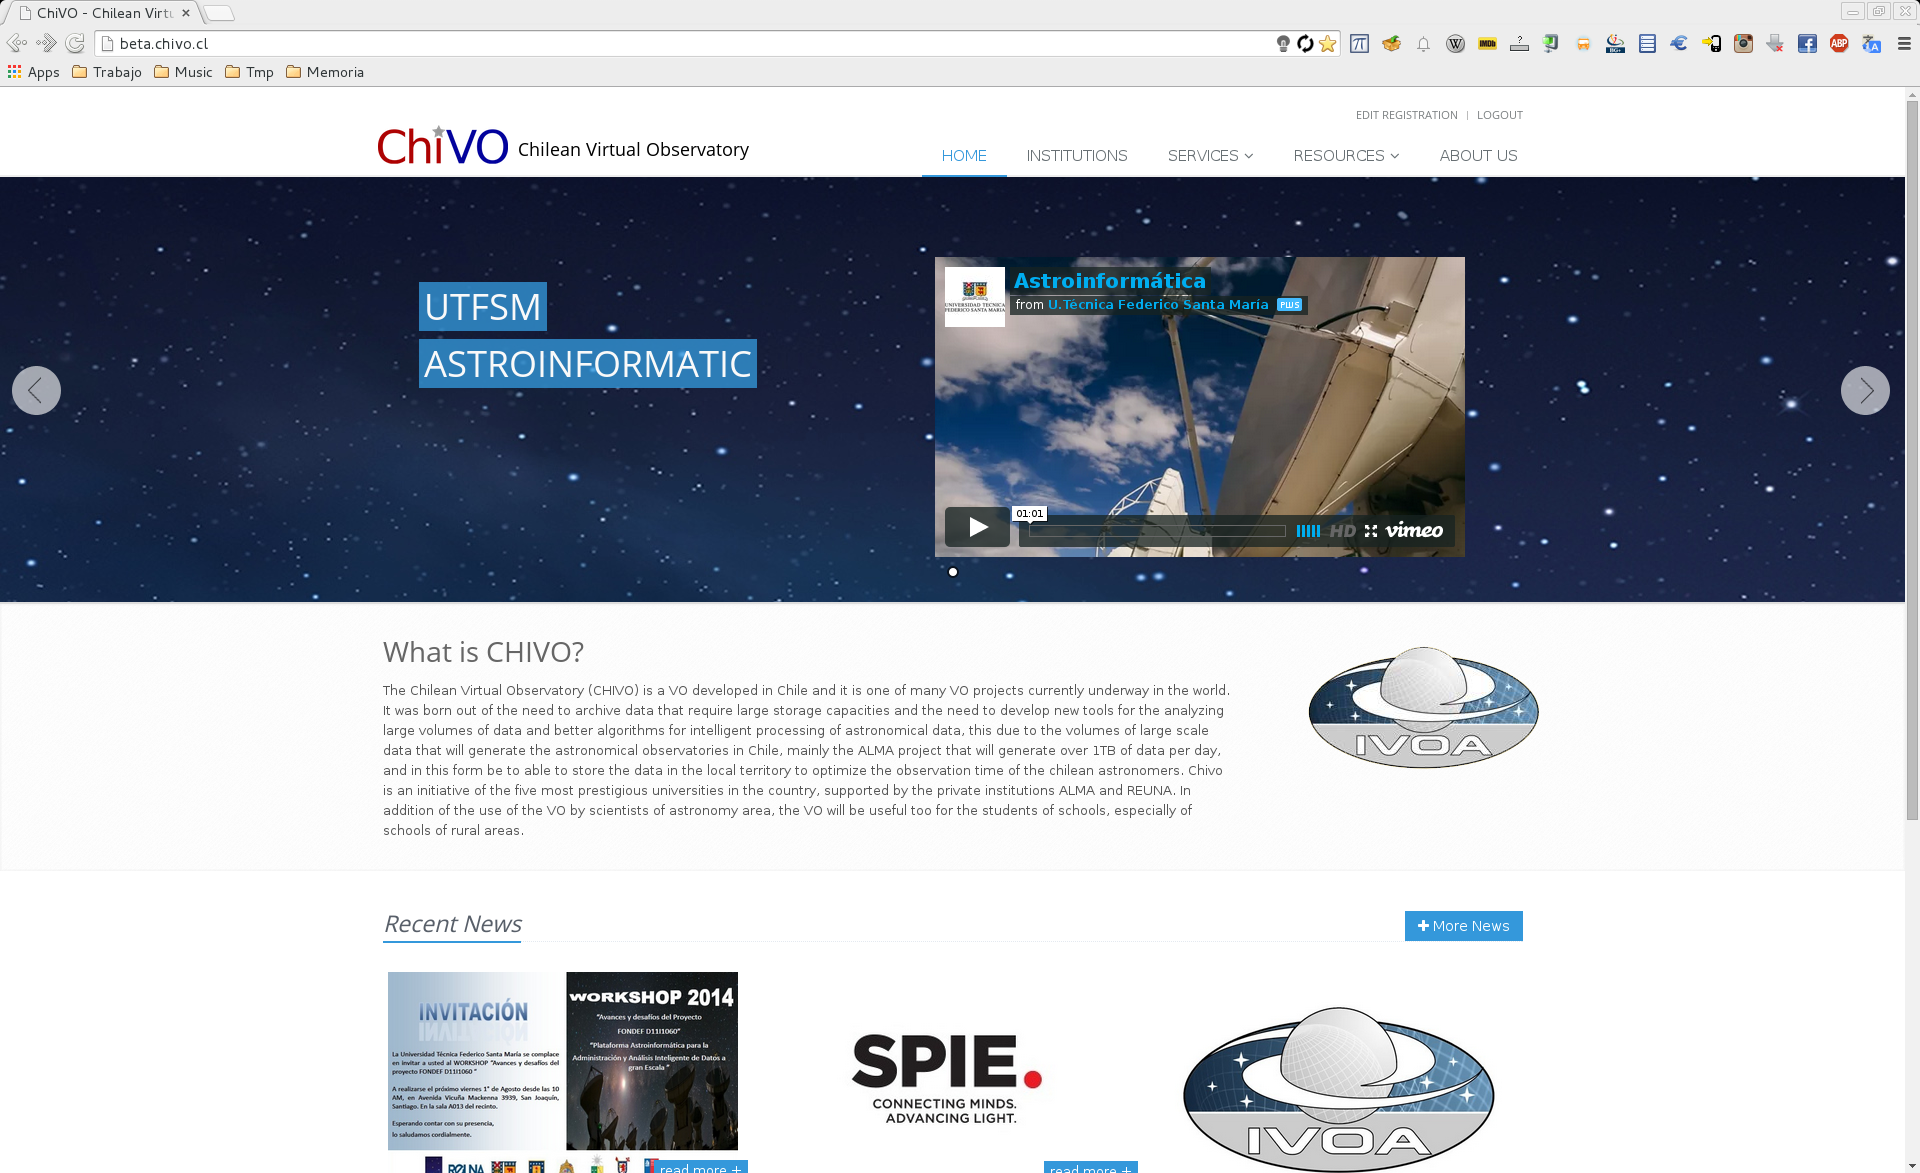
\includegraphics[scale=.2]{img/chivo}
    \end{center}
    \caption{Sitio del \emph{Chilean Virtual Observatory} en su
      versión beta.}\label{img:chivo}
\end{figure}

Por otro lado, se encuentra una sección (\emph{services}) dedicada a
realizar diferentes tipos de búsquedas según los protocolos
recomendados por IVOA\footnote{International Virtual Observatory
Alliance: \url{http://www.ivoa.net/}.}. Aquí se encontrará
específicamente 3 búsquedas: \emph{Simple Cone Search}, \emph{Simple
Image Access} y \emph{Simple Spectral Access}, además de un tipo de
búsqueda denominada \emph{all search}, que busca cumplir con los
requerimientos del mandante de este proyecto (ALMA), y que tiene por
objetivo emular el servicio \emph{ALMA Science Archive
Query}\footnote{\url{https://almascience.nrao.edu/aq/}.}. Esta última
sección no se encuentra dentro del marco de esta segunda
implementación, pues está basada bajo los estándares IVOA. No
obstante, se puede observar algunos tipos de búsquedas que ya han sido
implementadas.

A continuación se describe el desarrollo de cada una de las búsquedas
actualmente soportadas por ChiVO.


\subsection{Simple Cone Search}

Para acceder a esta búsqueda, se debe ingresar al menú superior
\emph{services} y seleccionar la opción \emph{cone search}, o ir
directamente a la dirección
\url{http://beta.chivo.cl/query/conesearch}. Allí se desplegará un
formulario con los datos requeridos para realizar la búsqueda, como se
muestra en la Fig.\ref{img:scs}.

\begin{figure}[ht!]
    \begin{center}
	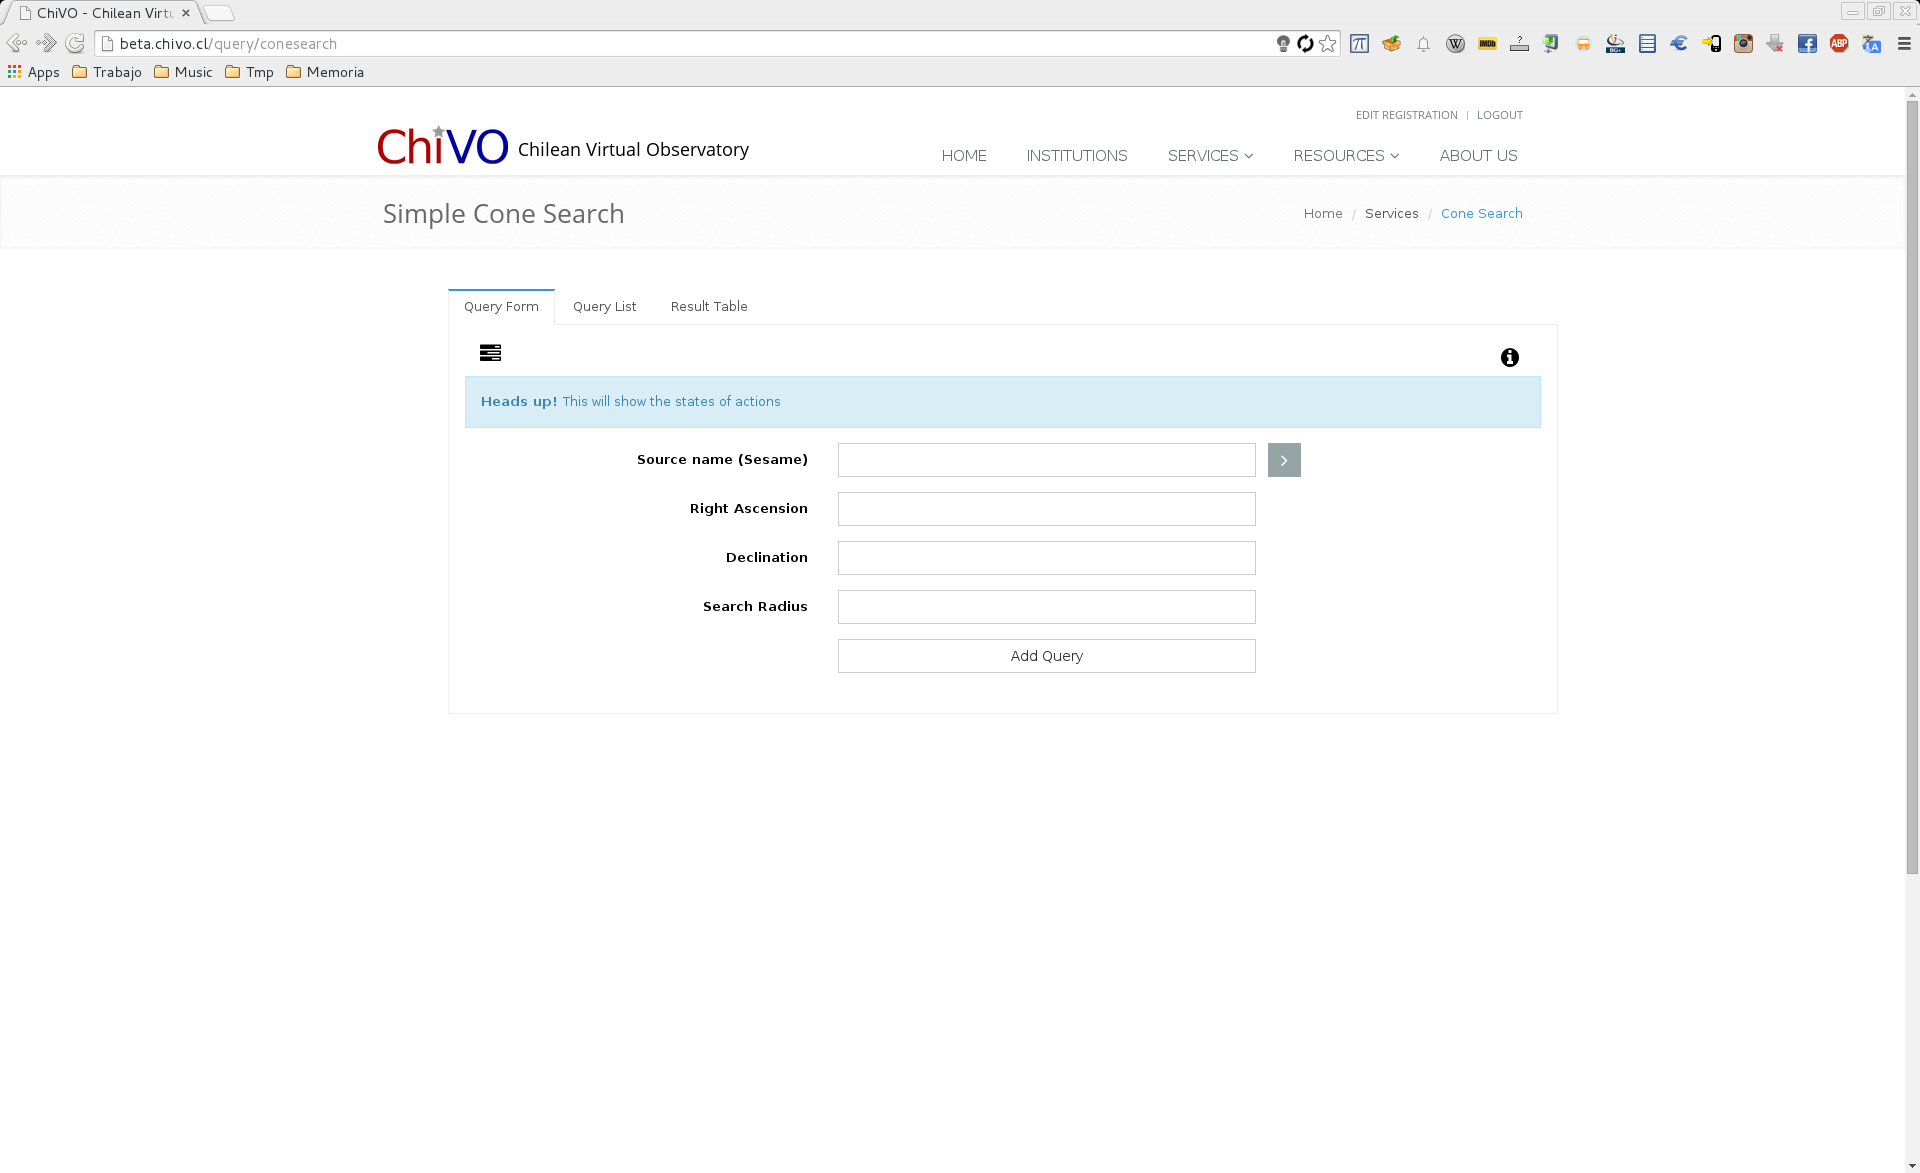
\includegraphics[scale=.2]{img/scs}
    \end{center}
    \caption{\emph{Simple Cone Search}.}\label{img:scs}
\end{figure}

Esta vista, tiene la característica de estar separada en 3 pestañas:
\emph{Query Form} (formulario de consulta), \emph{Query List} (lista
de consultas) y \emph{Result Table} (tabla de resultados). En las dos
primeras se podrá encontrar un ícono con la letra ``i'', el cual tiene
por objetivo mostrar una breve descripción que ayude al usuario a
entender qué significa cada campo. Si se presiona este ícono, los
campos en el formulario tomarán otro color, y con sólo posicionar el
cursor del ratón sobre uno de ellos se desplegará la ayuda. Además,
justo bajo el ícono de información se deplegará un mensaje por cada
acción ejecutada. En un comienzo, el primer mensaje resaltado será
\emph{Heads up! This will show the states of actions} (¡Ayuda! Esto
mostrará los estados de las acciones), avisando que allí se mostrará
una pequeña reseña por cada acción ejecutada.

A continuación se describirá el funcionamiento desarrollado para cada
una de las pestañas en esta búsqueda.

\begin{description}
  \item [Query Form:] este formulario de consulta permite ingresar los
    datos necesarios para poder realizar la búsqueda. Una vez
    ingresado los campos, se debe presionar el botón \emph{Add Query}
    (agregar consulta) para agregar la consulta a la lista de
    consultas. Una vez hecho esto, se debe pasar a la siguiente
    pestaña, \emph{Query List}. Los campos presentes en este
    formulario son:
    \begin{description}
      \item [Source name (Sesame):] corresponde a un resolvedor de
	nombres. Los objetos astronómicos poseen en su mayoría un
	nombre común de fácil aprendizaje, el cual puede ser ingresado
	en este campo y automáticamente el sistema completará los
	datos de RA \& DEC. Actualmente se utiliza el Sesame de
	{\ldots}, pero se trabaja en la construcción de uno propio.
      \item [Right Ascension:]
      \item [Declination:]
      \item [Search Radius:]
    \end{description}
  \item [Query List:]
    \begin{description}
      \item [Sources:]
    \end{description}  
  \item [Result Table:]
\end{description}  

\subsection{Simple Image Access}

Fig.~\ref{img:sia}

\begin{description}
  \item [Query Form:]
  \item [Query List:]
  \item [Result Table:]
\end{description}  

\begin{figure}[ht!]
    \begin{center}
	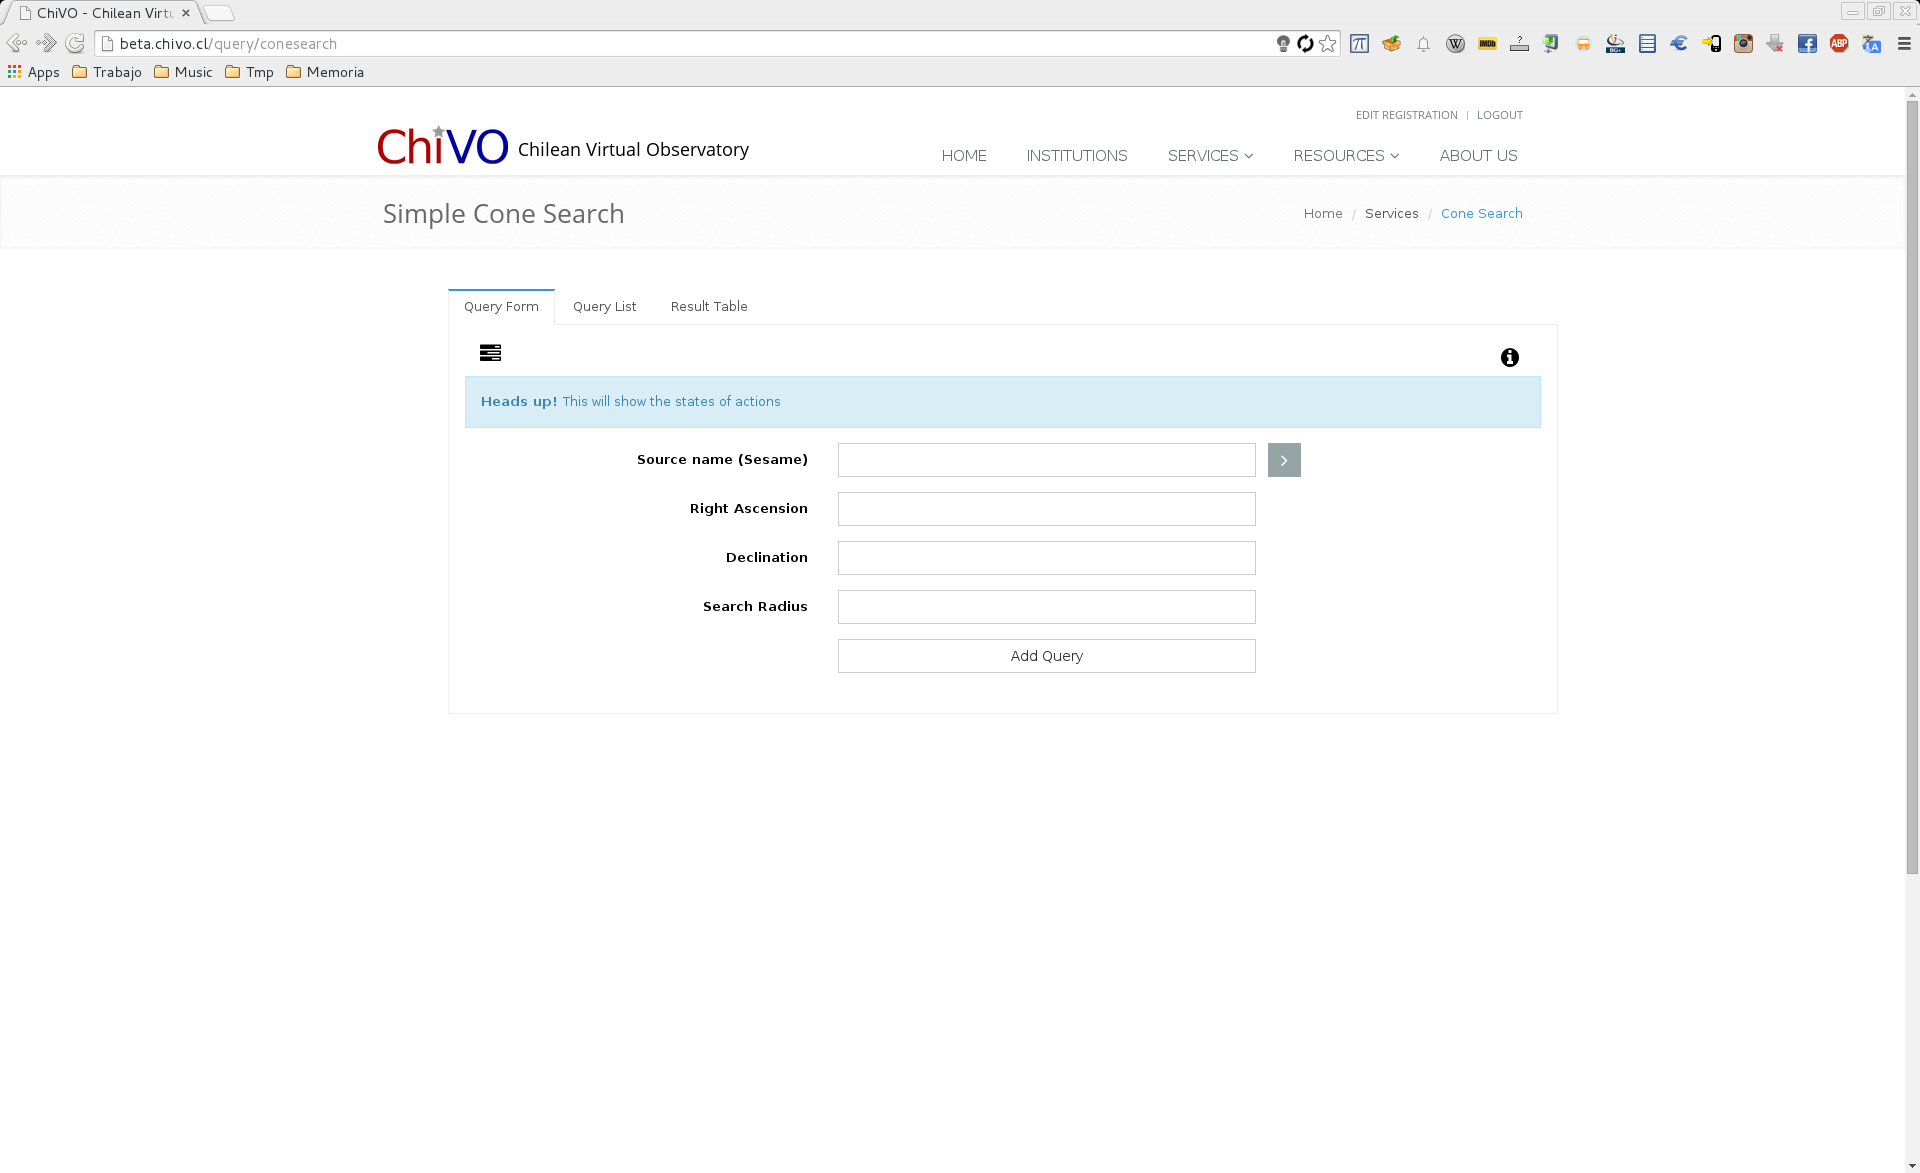
\includegraphics[scale=.2]{img/sia}
    \end{center}
    \caption{\emph{Simple Image Access}.}\label{img:sia}
\end{figure}



\subsection{Simple Spectral Access}

Fig.~\ref{img:ssa}

\begin{figure}[ht!]
    \begin{center}
	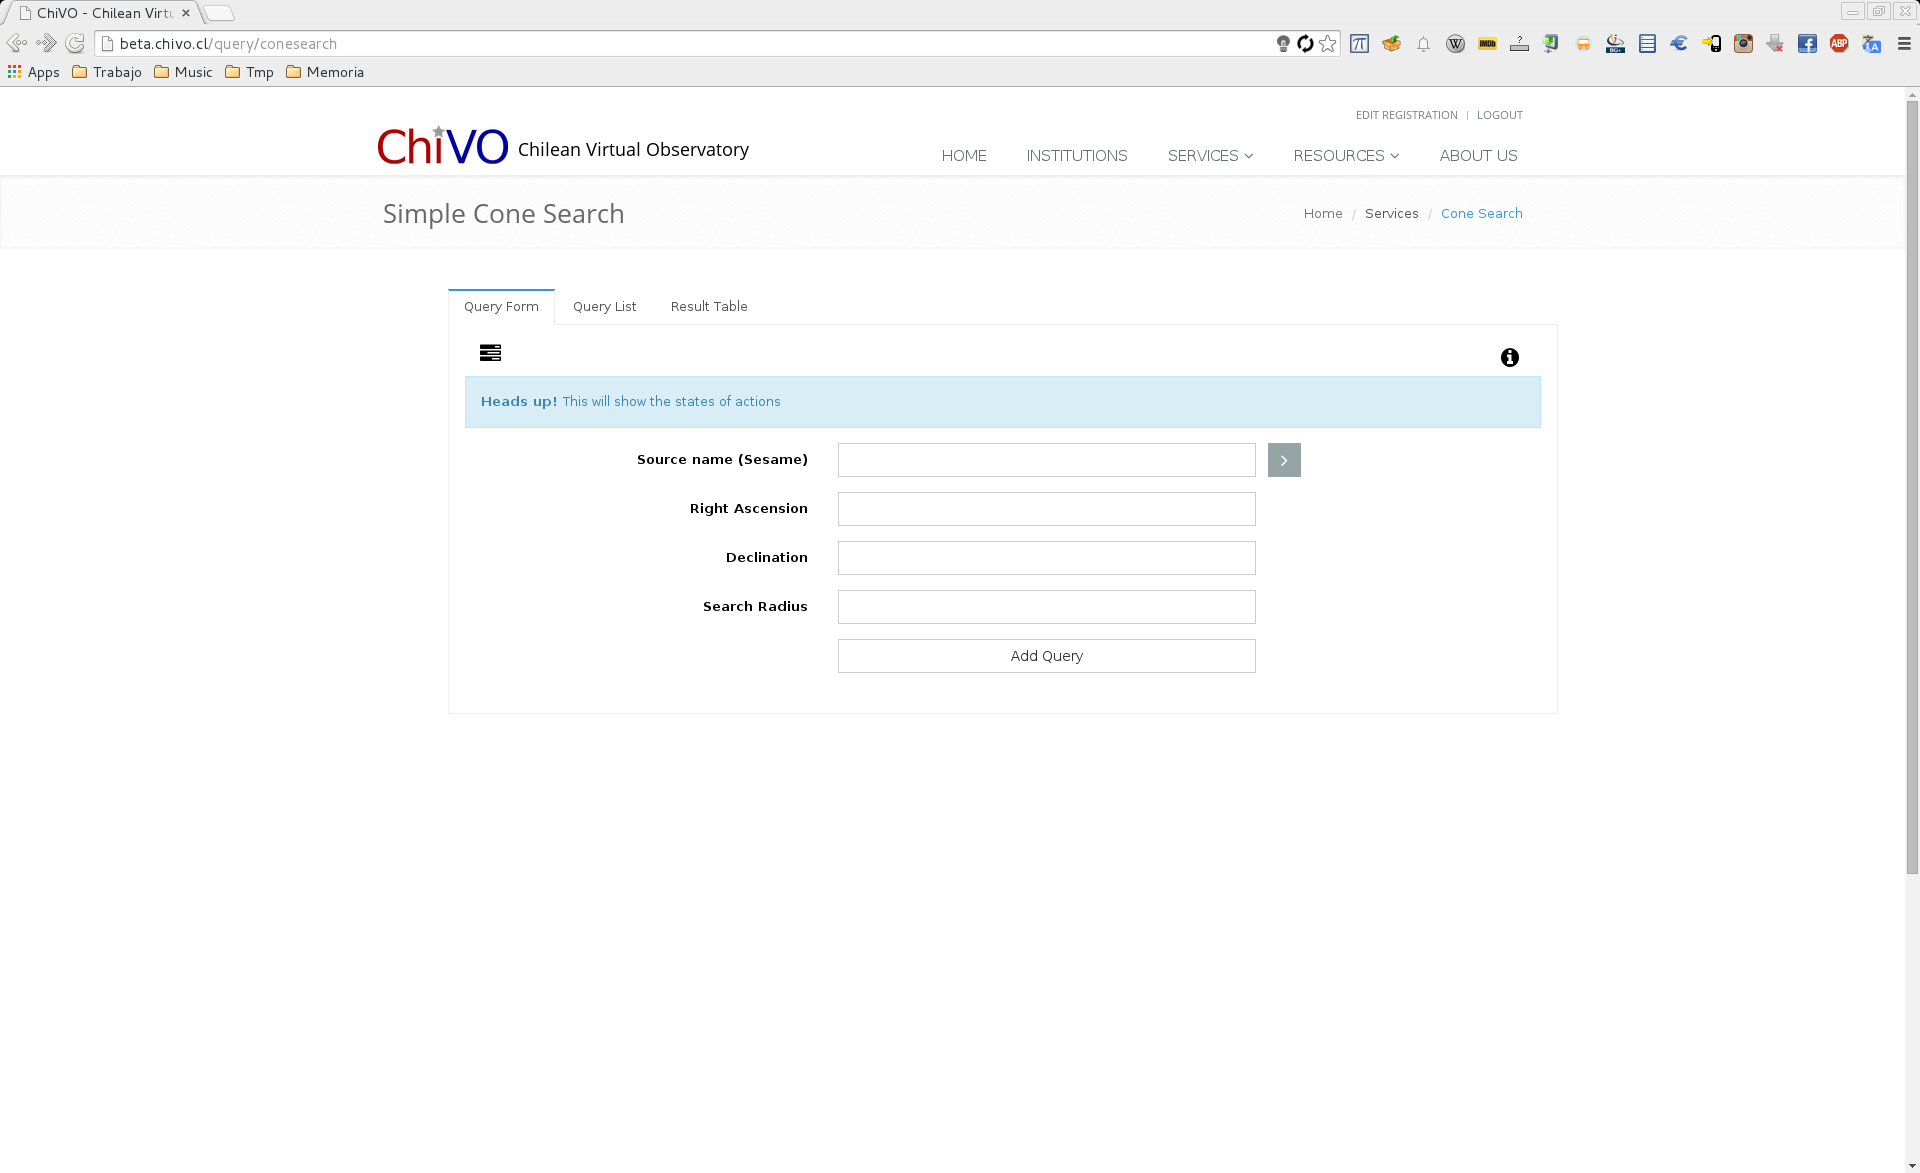
\includegraphics[scale=.2]{img/ssa}
    \end{center}
    \caption{\emph{Simple Spectral Access}.}\label{img:ssa}
\end{figure}

